\section{Overview of the Approach}
\label{sec-overview}

%%%%%%%%%%%%%%%
\begin{figure*}[tb!]
\vspace{-1ex}
\centerline{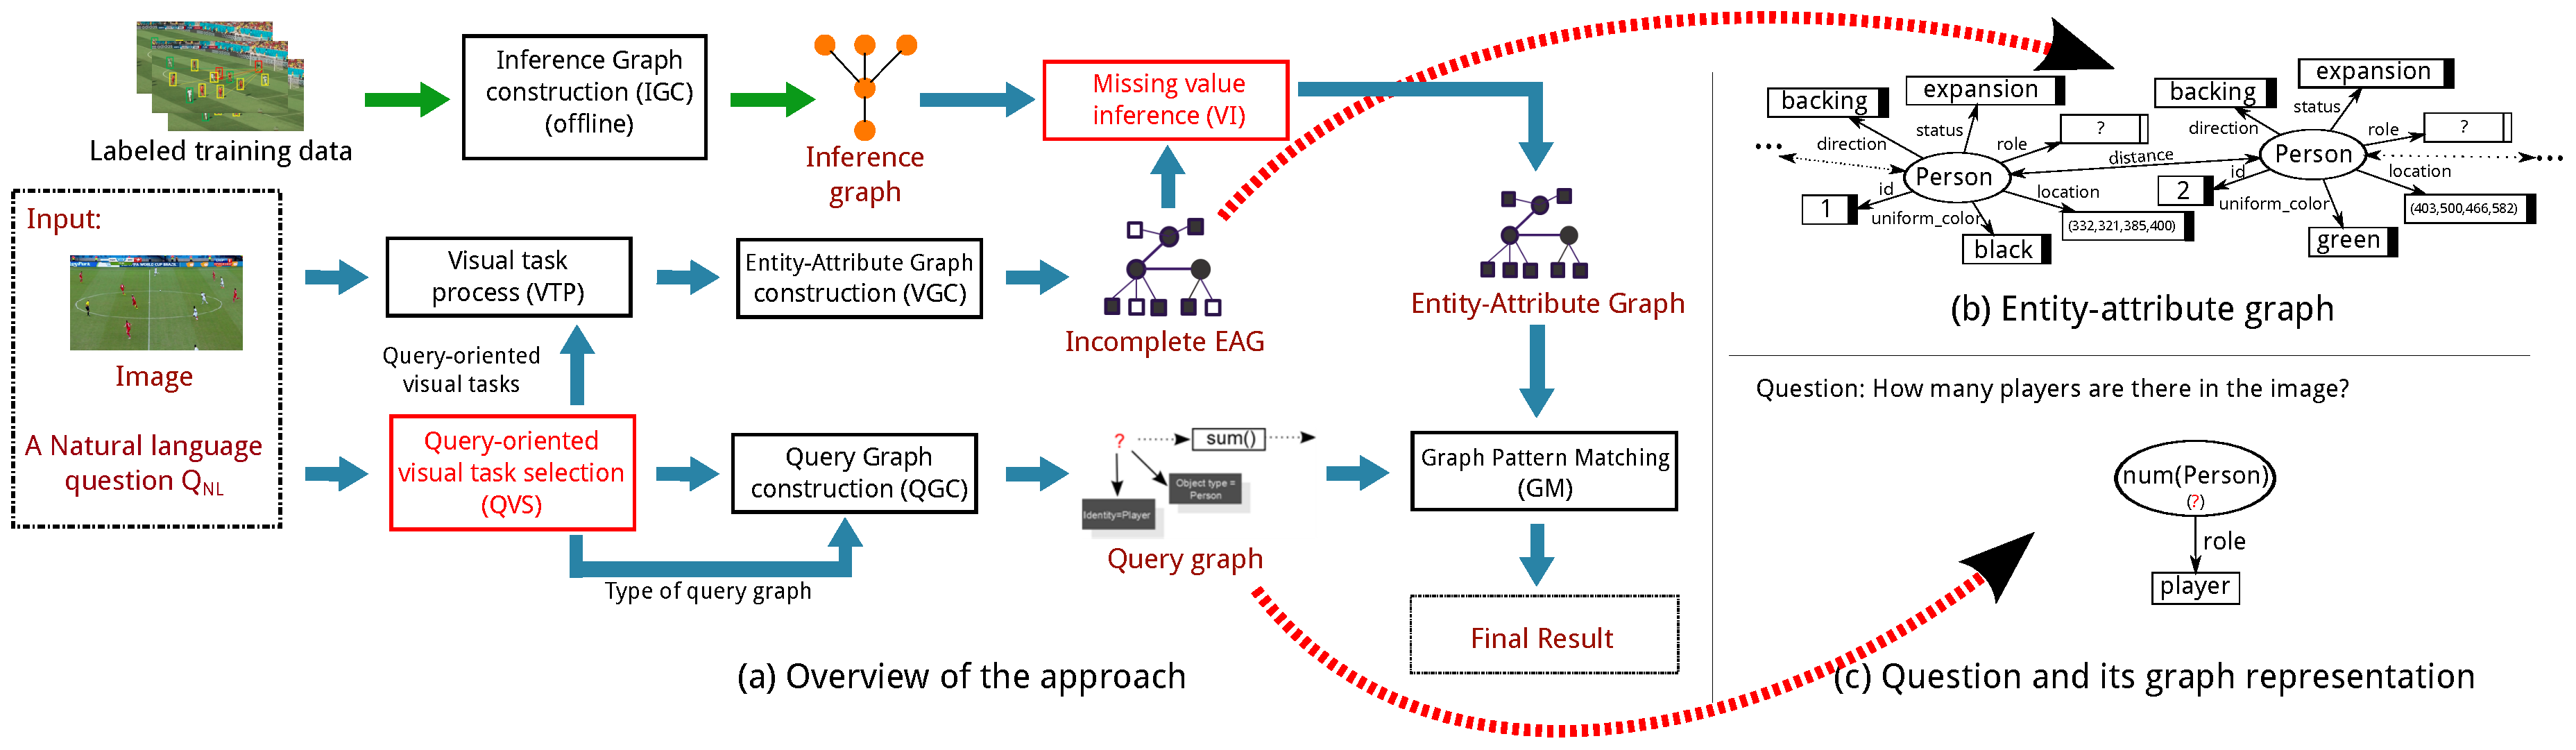
\includegraphics[scale=0.28]{overview.eps}}
\caption{\color{red}Overview of our approach, and graph-based representation of images and questions} \label{fig-overview}
\vspace{-2ex}
\end{figure*}
%%%%%%%%%%%%%%%%

We start from representations of images and questions, followed by the overview of our approach.


\subsection{Representation of Images and Questions}
\label{sec-representation}

We use the same representations as~\cite{peixi2019}. To make the paper self-contained, we cite them as follows (rephrased). 

\stitle{Entity-Attribute Graphs.} Entities are typically defined as objects or concepts that exist in the real world. An entity often carries attributes, that describe features of the entity. \looseness=-1

Assume a set ${\cal E}$ of entities, a set ${\cal D}$ of values, a set ${\cal P}$ of predicates indicating attributes of entities and a set $\Theta$ of types. 
Each entity $e$ in ${\cal E}$ has a {\em unique ID} and a {\em type} in $\Theta$.

An {\em entity-attribute} graph, denoted as \kw{EAG}, is a set of triples $t = (s, p, o)$, where {\em subject} $s$ is an entity in ${\cal E}$, $p$ is a {\em predicate} in ${\cal P}$, and {\em object} $o$ is either an entity in ${\cal E}$ or a value $d$ in ${\cal D}$. It can be represented as a directed edge-labeled graph $\eag=(V, E)$, such that (a) $V$ is the set of nodes consisting of $s$ and $o$ for each triple $t = (s, p, o)$; and (b) there is an edge in $E$ from $s$ to $o$ labeled by $p$ for each triple $t = (s, p, o)$. \looseness=-1


\eat{%20190305
We consider two types of equality:

\noindent (a) {\em node identity} on ${\cal E}$: $e_1\Leftrightarrow e_2$ if entities $e_1$ and $e_2$ have the same ID, \ie they refer to the same entity; and 

\noindent (b) {\em value equality} on ${\cal D}$: $d_1 = d_2$ if they are the same value.

In $\eag$, $e_1$ and $e_2$ are represented as the same node if $e_1\Leftrightarrow e_2$; 
similarly for values $d_1$ and $d_2$ if $d_1=d_2$.
}%20190305


An image can be represented as an \kw{EAG} with detected objects along with their detected attributes, and relationships among objects. This can be achieved via a few visual tasks. While \kw{EAG} generated directly after image processing is often incomplete, \ie it may miss some crucial information to answer queries. We hence refer to {\em entity-attribute graphs} with incomplete information as {\em incomplete entity-attribute graphs}, and associate nodes with white rectangles, to indicate the missing value of an entity or attribute in \kw{EAG}. Figure~\ref{fig:example}(b) is an {\em incomplete entity-attribute graph}, in which square nodes representing person roles are associated with white rectangle. 

\stitle{Query Graphs.}  A query graph $Q(u_o)$ is a set of triples
$(s_Q, p_Q, o_Q)$, where $s_Q$ is either a variable $z$ or a function $f(z)$ taking $z$ as parameter, $o_Q$ is one of a value $d$ or $z$ or $f(z)$, and $p_Q$ is a predicate in ${\cal P}$. Here function $f(z)$ is defined by users, and variable $z$ has one
of three forms: (a) {\em entity variable} $y$, to map to an entity, (b)
{\em value variable} $y*$, to map to a value, and (c) {\em wildcard} $\_y$, to
map to an entity. Here $s_Q$ can be either $y$ or $\_y$, while $o_Q$ can
be $y$, $y*$ or $\_y$. Entity variables and wildcard carry a {\em type},
denoting the type of entities they represent. 

A query graph can also be represented as a graph such
that two variables are represented as the same node if they
have the same name of $y$, $y*$ or $\_y$; similarly for functions $f(z)$ and values $d$.
We assume \kwlog that $Q(x)$ is connected, \ie there exists
an undirected path between $u_o$ and each node in $Q(u_o)$.
In particular, $u_o$ is a designated node in $Q(u_o)$, denoting the query focus and labeled by ``?''. %denoting an entity. Introduce functions.  \looseness=-1
Take Fig.~\ref{fig-overview}(c) as example. It depicts a query graph that is generated from query ``{\em How many players are there in the image?}''. Note that the ``query focus'' $u_o$ carries a function \kw{num}() that calculates the total number of {\em person} entities with {\em role} ``player''. 


\subsection{Approach Overview}
\label{sec-architecture}

% %%%%%%%%%%%%%%%
% \begin{figure*}[tb!]
% \vspace{-1ex}
% \centerline{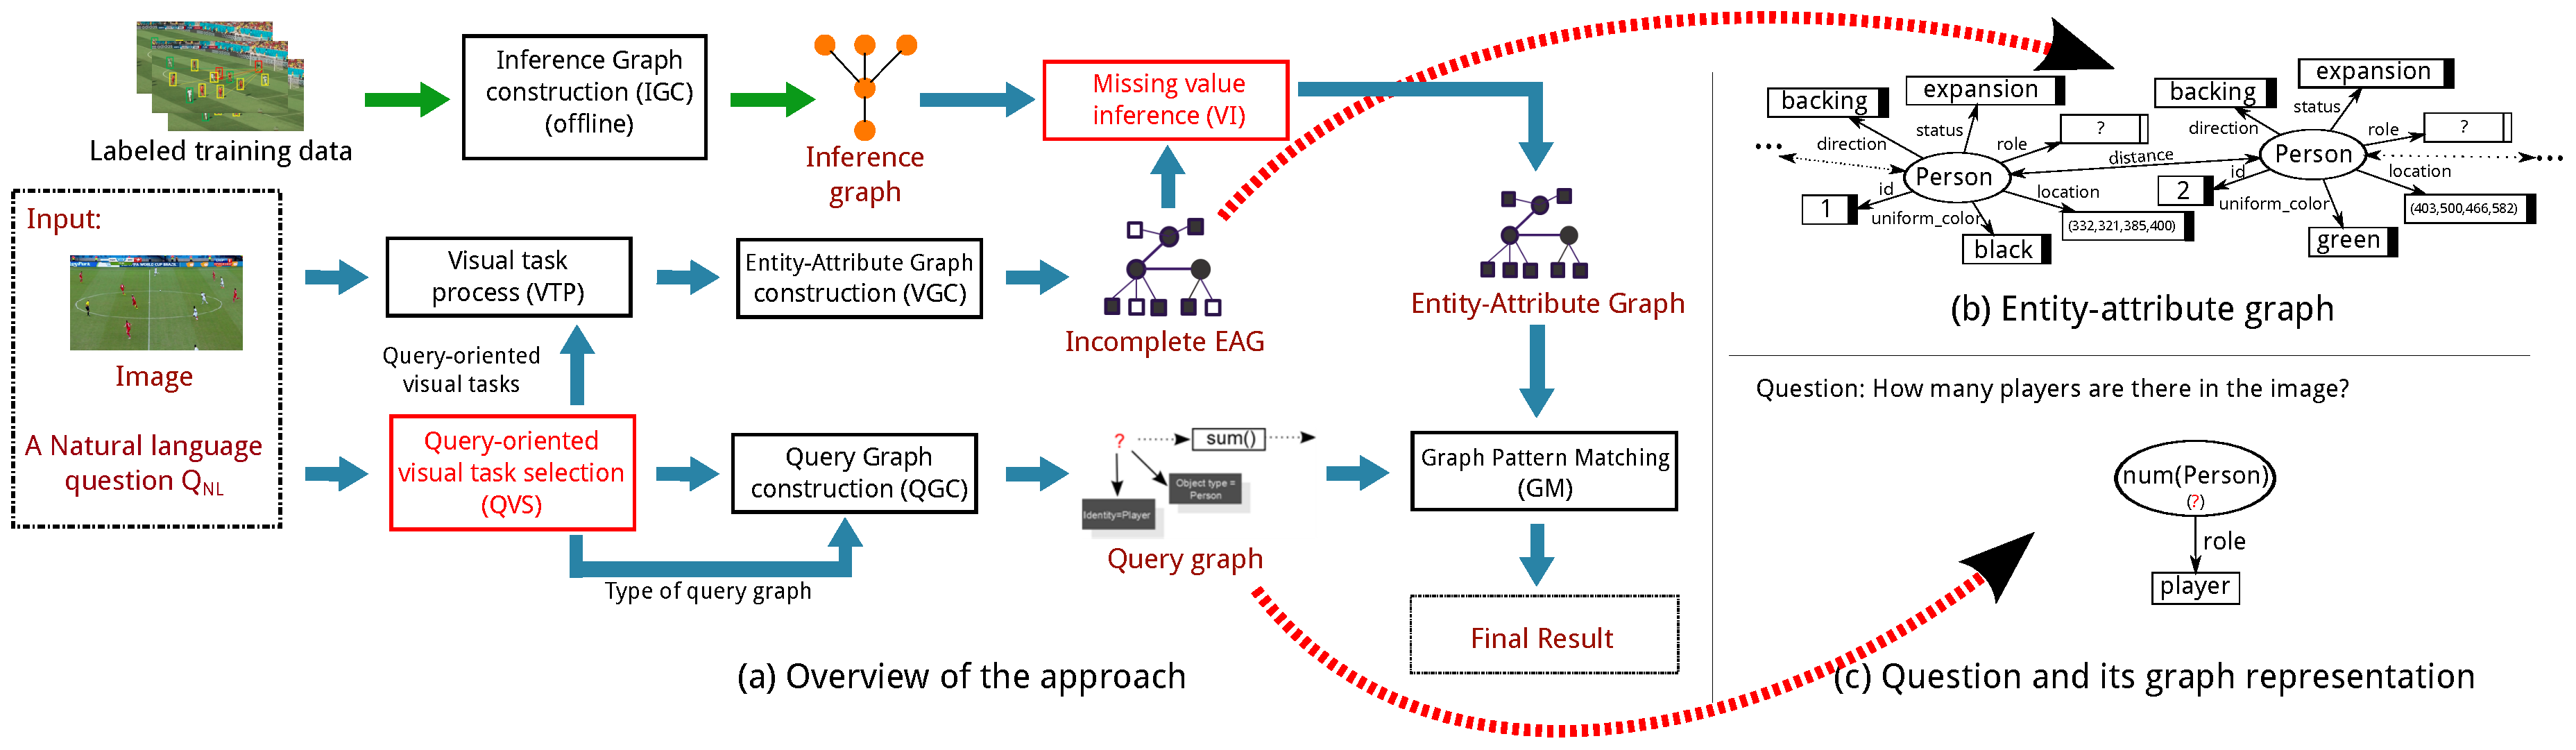
\includegraphics[scale=0.28]{overview.eps}}
% \caption{Overview of our approach, Entity Attribute Graph and Queries} \label{fig-overview}
% \vspace{-2ex}
% \end{figure*}
% %%%%%%%%%%%%%%%%


\eat{
Along the same lines as representations for images and questions, and graph pattern matching for question answering, raised in~\cite{peixi2019}, we propose a comprehensive approach as modeling of the \vqa problem. %answer a set of typical questions regarding soccer matches. 
}

Figure~\ref{fig-overview}(a) presents the overview of our approach. In a nutshell, our approach takes an image and a natural language question $Q_{NL}$ as input, and answers questions with seven modules as following. (1) Upon receiving a question $Q_{NL}$, module \kw{QVS} identifies a set of visual tasks that are query-oriented and category of the query graph that corresponds to the input question, and passes tasks and category to modules \kw{VTP} and \kw{QGC}, respectively. (2) Guided by the list of tasks, module \kw{VTP} conducts visual tasks over the input image, and returns identified objects along with their attributes to module \kw{VGC}. (3) Module $\kw{VGC}$ constructs an entity-attribute graph $\eag$, by using identified objects and their attributes. Note that $\eag$ may be incomplete and hence unable to answer questions. (4) When $\eag$ is incomplete, module \kw{VI} infers missing value with a classifier $G_I$, denoted as {\em inference graph}, and produces an updated \kw{EAG} for question answering. (5) Module \kw{QGC} takes category of the query graph as input, and generates a query graph $Q(u_o)$. (6) After $Q(u_o)$ and $\eag$ are generated, module $\kw{GM}$ is invoked for matching computation, and returns final result. (7) In contrast to online computation that are processed by above modules, the module \kw{IGC} constructs {\em inference graphs} using labeled training data, offline. \looseness=-1

{\color{red} As some modules employ existing techniques, to emphasize our novelty, we will elaborate modules $\kw{VA}$ and $\kw{VGA}$ in Section~\ref{sec-understanding}, modules \kw{IGC} and \kw{VI} in Section~\ref{Inference}, and module \kw{GM} in Section~\ref{Query Answering} with more details. \looseness=-1}